\documentclass[a4paper,12pt]{report}
\usepackage[a4paper, portrait, margin=0.5in]{geometry}
\usepackage[utf8]{inputenc}
\usepackage{graphicx}
\usepackage{dsfont}
\usepackage{amsmath}
\usepackage{esint}
\usepackage{mathtools}
\usepackage{cancel}
\usepackage{bbold}
\usepackage{wrapfig}
\usepackage{subcaption}
\usepackage{listings}
\usepackage{xcolor}		
\usepackage{systeme}
\usepackage{soul}
\usepackage{ amssymb }
\usepackage{url}
\usepackage{verbatim}
\usepackage{hyperref}
\setcounter{secnumdepth}{3}
\setcounter{tocdepth}{3}


% Title Page
\title{Introduction to Type 1 Chebyshev filters}
\author{Alessandro Marcelli}


\begin{document}
\maketitle

\tableofcontents

\newpage

\section{Low-pass Type 1 Chebyshev filters}

Type 1 Chebishev low pass filters are characterized by a very small transient band, at the price of oscillations in the passing band. The higher the filter's oreder, the smaller the transient band is and the more oscillations in passing band we have.  

\begin{figure}[!htb]
	\centering
	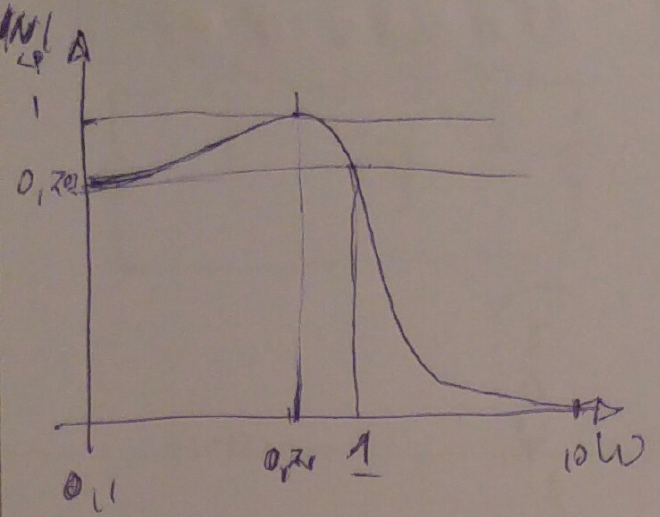
\includegraphics[width=.3\textwidth]{pictures/escheb.png}
	\caption{\label{lul} \small Example of a Low-pass Chebyshev filter}
\end{figure}


A filter of the n-th order is characterized by the following transfer function
\begin{align}
|H_{LP}^{(n)}(j\omega)|^2 = \frac{H_0^2}{1 + \epsilon^2\cdot C_n^2(\omega)}
\end{align}
where
\begin{enumerate}
\item $\omega = 2\pi f$
\item $H_0$ is the \textbf{maximum amplification in the filter's passing band}
\item $\epsilon$ is the \textbf{ripple factor}, whose contribute to the max amplitude in the passing band is given by 
\begin{align}
	k_p &= 20 \cdot \log_{10}(\sqrt{1 +\epsilon^2}) &[dB]
\end{align}

\item $C_n(\omega)$ is the \textbf{n-th order Chebyshev polynomial} (which can be found tabulated \cite{cheby}), where \textbf{n} corresponds to the filter order, which are defined as such 
\end{enumerate}
\begin{align}
	C_n(\omega) &= cos(n \cdot arccos(\omega))  &\omega &\in [0,1]\\
	C_n(\omega) &= cos(n \cdot arccosh(\omega)) &\omega &\geq 1
\end{align}  

More than $H_{LP}^{(n)}(j\omega)$ it's usually preferred the \textbf{normalized transfer function}, defined as
\begin{align}
|N_{LP}^{(n)}(j\omega)|^2=\frac{|H_{LP}^{(n)}(j\omega)|^2}{H_0^2} = \frac{1}{1 + \epsilon^2\cdot C_n^2(\omega)}
\end{align}

\section{Pole calculation}

Poles for Type 1 Chebyshev lay along the left side of an ellpise, with one real for odd values of n.  
Studying the tranfer function the following expression for pole calculation can be derived:

\begin{align}
	p_k &= \sigma_k + j \omega_k\\
	\sigma_k &= -sin(u_k) \cdot sinh(v)\\
	\omega_k &= +cos(u_k)\cdot cosh(v)\\
	u_k & = \frac{2k-1}{2n}\cdot \pi\\
	v &= \frac{1}{n}\cdot arcsinh \left( \frac{1}{\epsilon} \right)
\end{align}


\newpage
\subsection{Example: 7th order low-pass filter with $\epsilon=1$}

For a 7th order low-pass filter with $\epsilon=1$ the normalized transfer function becomes

\begin{align}
	|N_{LP}^{(7)}(j\omega)|^2 = \frac{1}{1 + (64\omega^7 - 112 \omega^5 + 56\omega^3 - 7\omega)^2}
\end{align}

Using the given formulas we get

\begin{align}
	u_1 & = \frac{1}{14}  \cdot \pi\\
	u_2 & = \frac{3}{14}  \cdot \pi\\
	u_3 & = \frac{5}{14}  \cdot \pi\\
	u_4 & = \frac{1}{2}   \cdot \pi\\
	u_5 & = \frac{9}{14}  \cdot \pi\\
	u_6 & = \frac{11}{14} \cdot \pi\\
	u_7 & = \frac{13}{14} \cdot \pi\\
	v &= 0.1259
\end{align}

This leads to the following 7 poles 

\begin{align}
	p_1 &= -0.0281 + j \cdot 0.9827 \\
	p_2 &= -0.0787 + j \cdot 0.7880 \\
	p_3 &= -0.1137 + j \cdot 0.4373 \\
	p_4 &= -0.1262				\\
	p_5 &= -0.1137 - j \cdot 0.4373 \\
	p_6 &= -0.0787 - j \cdot 0.7880 \\
	p_7 &= -0.0281 - j \cdot 0.9827
\end{align}

\begin{figure}[!htb]
	\centering
	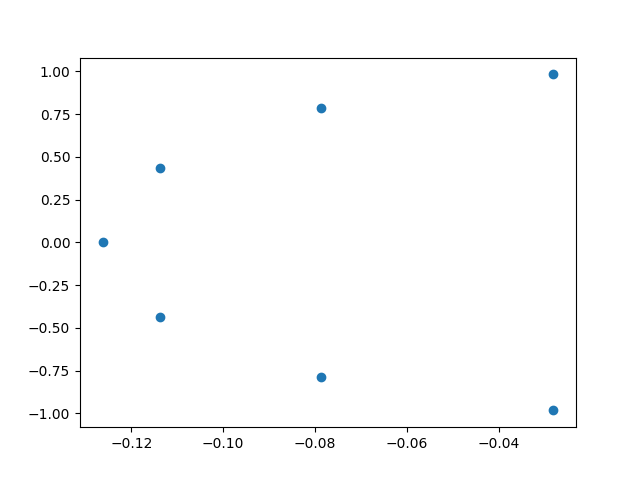
\includegraphics[width=.5\textwidth]{pictures/n=7_epsilon=1.0.png}
	\caption{\label{lul} \small Poles on the plane}
\end{figure}

\newpage

\section{Chebyshev tables}

For the calculation of normalized impedences, one usually consults the Chebyshev tables \cite{tables}, characterized by the filter's order and desired \textbf{ripple factor} $\epsilon$. 

As an example, here are some table values for $\epsilon=1.0$

\begin{center}
	\begin{tabular}{||c c c c c c c c c c||} 
		\hline
		N & $g_1$  & $g_2$  & $g_3$  & $g_4$  & $g_5$  & $g_6$  & $g_7$  & $g_8$ & \dots \\ [0.5ex] 
		\hline
		\vdots &&&&&&&&&\\
		\hline
		 5  & 3.4817 & 0.7618 & 4.5381 & 0.7618 & 3.4817 & 1.0000 &   &  & \\ 
		\hline
		 6  & 3.5045 & 0.7684 & 4.6061 & 0.7929 & 4.4641 & 0.6033 & 5.8095 &  & \\
		\hline
		7  & 3.5182 & 0.7723 & 4.6386 & 0.8039 & 4.6386 & 0.7723 & 3.5182 & 1.0000 & \\
		\hline 
		\vdots &&&&&&&&&\\
		\hline
	\end{tabular}
\end{center}

Let's see how the examples above can be interpreted using a LC ladder configuration.

\begin{enumerate}
	\item 5th order filter
	
	\begin{tabular}{||c c c c c c c ||} 
		\hline
		N & $C_2$  & $L_2$  & $C_3$  & $L_3$  & $C_1$  & $Z_{out}$\\ [0.5ex] 
		\hline
		5  & 3.4817 & 0.7618 & 4.5381 & 0.7618 & 3.4817 & 1.0000\\ 
		\hline
	\end{tabular}

	\begin{verbatim}
		--------------L_2-------L_3------------------
		|         |         |         |         |
		Gen       C_1       C_2       C_3       R_out
		|         |         |         |         |
		---------------------------------------------
	\end{verbatim}
	
	\item 6th order filter
	
	\begin{tabular}{||c c c c c c c c||} 
		\hline
		N & $C_1$  & $L_1$  & $C_2$  & $L_2$  & $C_3$ & $L_3 $ &$Z_{out}$\\ 	[0.5ex] 
		\hline
	 	6  & 3.5045 & 0.7684 & 4.6061 & 0.7929 & 4.4641 & 0.6033 & 5.8095\\ 
		\hline
	\end{tabular}

	\begin{verbatim}
		----L_1-------L_2-------L_3------------------
		|         |         |         |         |
		Gen       C_1       C_2       C_3       R_out
		|         |         |         |         |
		---------------------------------------------
	\end{verbatim}
		\item 7th order filter
	
		\begin{tabular}{||c c c c c c c c c ||} 
			\hline
			N & $C_2$  & $L_2$  & $C_3$  & $L_3$  & $C_4$  & $L_4$  & $C_1$  & $Z_{out}$\\ [0.5ex] 
			\hline
			7  & 3.5182 & 0.7723 & 4.6386 & 0.8039 & 4.6386 & 0.7723 & 3.5182 & 1.0000\\ 
			\hline
		\end{tabular}

	\begin{verbatim}
		--------------L_2-------L_3-------L_4------------------
		|         |         |         |         |         |
		Gen       C_1       C_2       C_3       C_4       R_out
		|         |         |         |         |         |
		--------------------------------------------------------
	\end{verbatim}
\end{enumerate}

We can notice two thing:
\begin{enumerate}
	\item For odd order filters the second-to-last impedence in the table actually corresponds to the first net of the filter
	\item For even order filters one can't have the same input and output loads, so a scaling factor is mandatory
\end{enumerate}

\section{Components calculation}

The values for a n-th order filter with a specific \textbf{ripple factor} $\epsilon$ and a specific \textbf{output load} $Z_{out}$ are calculated denormalizing the values found in Chebyshev tables via the following equations:

\begin{align}
	C_i &= \frac{C_{i_{norm}} }{2\pi f_c \cdot Z_{out}}\\
	L_i &= \frac{L_{i_{norm}} \cdot Z_{out} }{2\pi f_c}\\
	R_{out} &=g_{n+1} \cdot Z_{out}
\end{align}

The term $g_{n+1}$ is the last impedence value on the n-th row of the table.

Let's take a look once again at the  $\epsilon = 1$ case, and choose
\begin{align}
	R_{out} &= 50 \ [\Omega]\\
f_c &= 1 \ [MHz]
\end{align}

\begin{enumerate}
	\item 5th order filter
		
		\begin{tabular}{||c c c c c c ||} 
			\hline
			$C_2 \;[nF]$  & $L_2 \;[\mu H]$  & $C_3 \;[nF]$  & $L_3 \;[\mu H]$  & $C_1 \;[nF]$  & $Z_{out} \;[\Omega]$\\ [0.5ex] 
			\hline
			11.083 & 6.0622 & 14.445 & 6.0622 & 11.083 & 50.000\\ 
			\hline
		\end{tabular}
	
	\item 6th order filter
		
		\begin{tabular}{||c c c c c c c||} 
			\hline
			$C_1\;[nF]$  & $L_1\;[\mu H]$  & $C_2\;[nF]$  & $L_2\;[\mu H]$  & $C_3\;[nF]$ & $L_3 \;[\mu H]$ &$Z_{out}\;[\Omega]$\\ 	[0.5ex] 
			\hline
			11.155 & 6.1147 & 14.662 & 6.3097 & 14.210 & 4.8009 & 290.48\\ 
			\hline
		\end{tabular}
			
	\item 7th order filter
	
		\begin{tabular}{||c c c c c c c c||} 
			\hline
			$C_2 \;[nF]$  & $L_2 \;[\mu H]$  & $C_3 \;[nF]$  & $L_3 \;[\mu H]$  &$C_4 \;[nF]$  & $L_4 \;[\mu H]$  & $C_1 \;[nF]$  & $Z_{out} 	\;[\Omega]$\\ [0.5ex] 
			\hline
			11.199 & 6.1458 & 14.765 & 6.3972 & 14.765 & 6.1458 & 11.199 & 50.000\\ 
			\hline
		\end{tabular}
\end{enumerate}

\section{Low-Pass to Band-pass conversion}

Low-pass and Band-pass filters are bound together by the following variable change
\begin{align}
	s = p + \frac{1}{p} \ ; \ p \in \mathbb{C}
\end{align}
This relation brings us two consequences:

\begin{enumerate}
	\item Studying the inductors' impedances one finds that
	\begin{align}
		Z_{LP}(s) = ks \rightarrow Z_{BP}(p) = kp + \frac{k}{p} \ ; \ p \in \mathbb{C}
	\end{align}
	This means that we have to add a capacitor in series to every inductor.  
	We can calculate the values using the following relation
	\begin{align}
		C_{s_k} = \frac{\Delta f_{rel}}{2\pi f_{mid} \cdot L_{k_{norm}} \cdot Z_{out}}
	\end{align}
	\item Conversely, studying the capacitors' conductances one finds that
	\begin{align}
		Y_{LP}(s) = ks \rightarrow Y_{BP}(p) = kp + \frac{k}{p} \ ; \ p \in \mathbb{C}
	\end{align}
	This means we have to put an inductor in parallel to each capacitor, which we can calculate with the following relation
	\begin{align}
		L_{p_k} = \frac{\Delta f_{rel} \cdot Z_{out}}{2\pi f_{mid} \cdot L_{k_{norm}}}
	\end{align}
\end{enumerate}
Following, as an example, the schematic for a 5th order Band-pass filter
\begin{verbatim}
--------------------------L_2---C_s_2-----------L_3---C_s_3------------------------------
|                 |   |                 |   |                 |   |         |
Gen               C_1 L_p_1             C_2 L_p_2             C_3 L_p_3     R_out
|                 |   |                 |   |                 |   |         |
-----------------------------------------------------------------------------------------
\end{verbatim}

\begin{center}
	\begin{tabular}{||c c||} 
	\hline
	1st net components &\\ [0.5ex] 
	\hline
	 $C_1 = 11.083 \;[nF]$ & $L_{1_{par}} = 31.352\;[nH]$\\ 
	\hline\hline
	2st net components &\\ [0.5ex] 
	\hline
	$L_2 = 6.0622\; [\mu H]$ & $C_{2_{ser}} = 57.317 \;[pF]$\\
	$C_2 = 11.083\; [nF]$ & $L_{2_{par}} = 31.352\; [nH]$\\
	\hline\hline
	3st net components &\\ [0.5ex] 
	\hline
	$L_3 = 6.0622\; [\mu H]$ & $C_{3_{ser}} = 57.317 \;[pF]$\\
	$C_3 = 14.445\; [nF]$ & $L_{3_{par}} = 24.054\; [nH]$\\
	\hline\hline
	Output load &\\ [0.5ex] 
	\hline
	$R_{out} = 50.000 \;[\Omega]$ &\\ 
	\hline\hline
\end{tabular}
\end{center}


\bibliographystyle{plain}
\bibliography{bibliography.bib}
\end{document}          
